\exercisesheader{}

% 23 - diamonds_1_ahss

\eoce{\qt{Diamonds, Part I\label{diamonds_1_ahss}} Prices of diamonds are determined by 
what is known as the 4 Cs: cut, clarity, color, and carat weight. The prices of 
diamonds go up as the carat weight increases, but the increase is not smooth. 
For example, the difference between the size of a 0.99 carat diamond and a 1 
carat diamond is undetectable to the naked human eye, but the price of a 1 
carat diamond tends to be much higher than the price of a 0.99 diamond. In this 
question we use two random samples of diamonds, 0.99 carats and 1 carat, each 
sample of size 23, and compare the average prices of the diamonds. In order to 
be able to compare equivalent units, we first divide the price for each diamond 
by 100 times its weight in carats. That is, for a 0.99 carat diamond, we divide 
the price by 99. For a 1 carat diamond, we divide the price by 100. The 
distributions and some sample statistics are shown below.\footfullcite{ggplot2} \\[1mm]
\begin{minipage}[c]{0.6\textwidth}
Conduct a hypothesis test to evaluate if there is a difference between the 
average standardized prices of 0.99 and 1 carat diamonds.  Include all steps of the ICCCC framework. \\[2mm]
\begin{tabular}{l c c }
\hline
        & 0.99 carats       & 1 carat\\
\hline  
Mean    & \$44.51          & \$56.81           \\
SD      & \$13.32          &\$16.13            \\
n       &23             & 23 \\
\hline
\end{tabular}
\end{minipage}%
\begin{minipage}[c]{0.4\textwidth}
\begin{center}
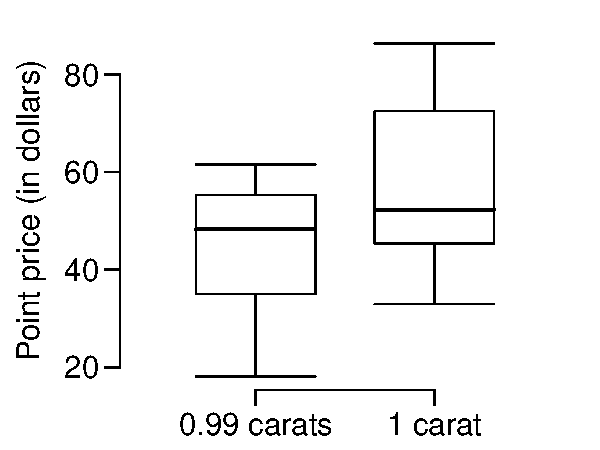
\includegraphics[width=0.85\textwidth]{ch_inference_for_means/figures/eoce/diamonds_1_ahss/diamonds_box.pdf}
\end{center}
\end{minipage}
}{}

% 24 - diamonds_2_ahss

\eoce{\qt{Diamonds, Part II\label{diamonds_2_ahss}} In Exercise~\ref{diamonds_1_ahss}, we 
discussed diamond prices (standardized by weight) for diamonds with weights 0.
99 carats and 1 carat. See the table for summary statistics, and then construct 
a 95\% confidence interval for the difference in means between the standardized 
prices of 0.99 and 1 carat diamonds. Include all steps of the ICCCC framework.
\begin{center}
\begin{tabular}{l c c }
\hline
        & 0.99 carats       & 1 carat\\
\hline  
Mean    & \$44.51          & \$56.81           \\
SD      & \$13.32          &\$16.13            \\
n       &23             & 23 \\
\hline
\end{tabular}
\end{center}
}{}

% 25 - chick_wts_linseed_horsebean

\eoce{\qt{Chicken diet and weight,
    Part I\label{chick_wts_linseed_horsebean}} \videosolution{ahss_eoce_sol-chick_wts_linseed_horsebean} Chicken farming is a multi-billion dollar industry,
and any methods that increase the growth rate of young
chicks can reduce consumer costs while increasing
company profits, possibly by millions of dollars.
An experiment was conducted to measure and compare
the effectiveness of various feed supplements on the
growth rate of chickens.
Newly hatched chicks were randomly allocated into six groups, 
and each group was given a different feed supplement.
Below are some summary statistics from this data set along
with box plots showing the distribution of weights by
feed type.\footfullcite{data:chickwts}

\noindent\begin{minipage}[c]{0.65\textwidth}
\begin{center}
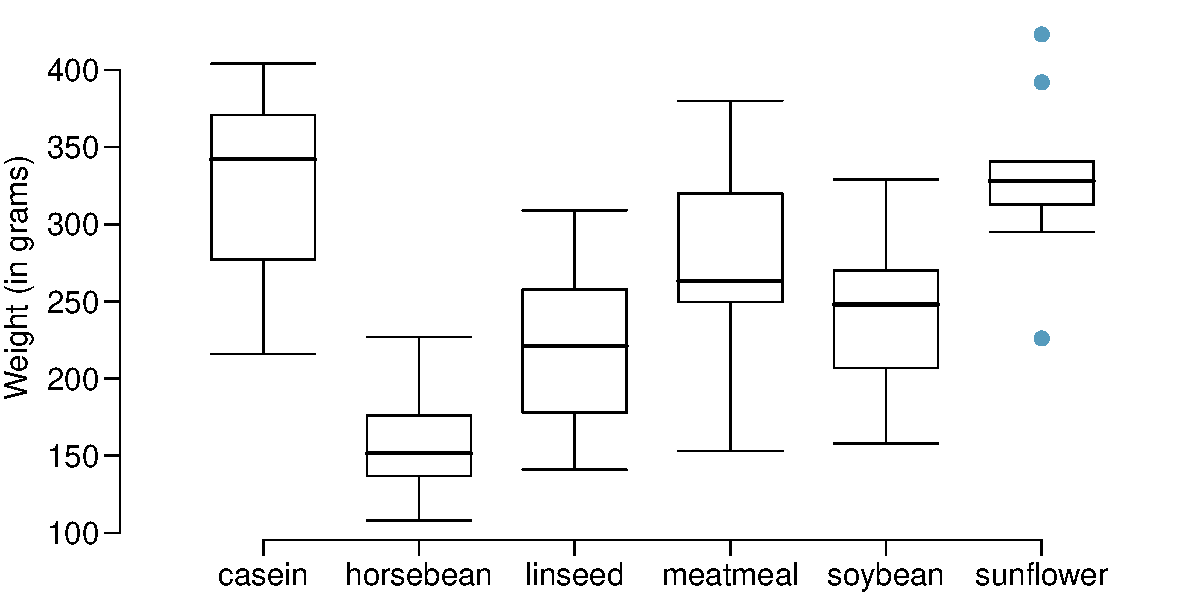
\includegraphics[width= \textwidth]{ch_inference_for_means/figures/eoce/chick_wts_linseed_horsebean/chick_wts_box.pdf}
\end{center}
\end{minipage}
\begin{minipage}[c]{0.35\textwidth}
{\footnotesize\begin{tabular}{l c c c}
\hline
            & Mean      & SD        & n \\
\hline
casein          & 323.58        & 64.43 & 12 \\
horsebean   & 160.20        & 38.63 & 10 \\
linseed         & 218.75        & 52.24 & 12 \\
meatmeal    & 276.91        & 64.90 & 11 \\
soybean         & 246.43        & 54.13 & 14 \\
sunflower       & 328.92        & 48.84 & 12 \\
\hline
\end{tabular}}
\end{minipage} 

\begin{parts}
\item Describe the distributions of weights of chickens that were fed linseed 
and horsebean.
\item Do these data provide strong evidence that the average weights of 
chickens that were fed linseed and horsebean are different? Use a 5\% 
significance level.
\item What type of error might we have committed? Explain.
\item Would your conclusion change if we used $\alpha = 0.01$?
\end{parts}
}{}

% 26 - fuel_eff_city

\eoce{\qt{Fuel efficiency of manual and automatic cars, Part I\label{fuel_eff_city}} 
Each year the US Environmental Protection Agency (EPA)
releases fuel economy data on cars manufactured in that year.
Below are summary statistics on fuel efficiency (in miles/gallon)
from random samples of cars with manual and automatic transmissions.
Do these data provide strong evidence of a difference between the
average fuel efficiency of cars with manual and automatic
transmissions in terms of their average city mileage?  
 \footfullcite{data:epaMPG}

\noindent\begin{minipage}[c]{0.38\textwidth}
\begin{center}
\begin{tabular}{l c c }
\hline
        & \multicolumn{2}{c}{City MPG} \\
\hline
        & Automatic     & Manual         \\
Mean    & 16.12         & 19.85      \\
SD      & 3.58          & 4.51       \\
n       & 26            & 26 \\
\hline
& \\
& \\
\end{tabular}
\end{center}
\end{minipage}
\begin{minipage}[c]{0.6\textwidth}
\begin{center}
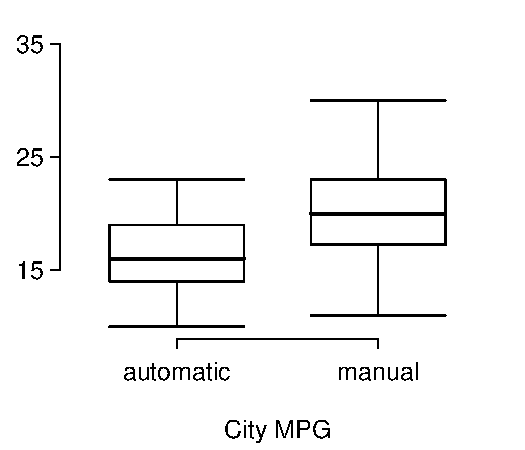
\includegraphics[width=0.7\textwidth]{ch_inference_for_means/figures/eoce/fuel_eff_city/fuel_eff_city_box.pdf}
\end{center}
\end{minipage}
}{}

% 27 - chick_wts_casein_soybean

\eoce{\qt{Chicken diet and weight, Part II\label{chick_wts_casein_soybean}} Casein is 
a common weight gain supplement for humans. Does it have an effect on chickens? 
Using data provided in Exercise~\ref{chick_wts_linseed_horsebean}, test the 
hypothesis that the average weight of chickens that were fed casein is 
different than the average weight of chickens that were fed soybean. If your 
hypothesis test yields a statistically significant result, discuss whether or 
not the higher average weight of chickens can be attributed to the casein diet. 
Conditions for inference were checked in Exercise~\ref{chick_wts_linseed_horsebean}.
}{}

% 28 - fuel_eff_hway

\eoce{\qt{Fuel efficiency of manual and automatic cars, Part II\label{fuel_eff_hway}} 
The table provides summary statistics on highway fuel economy
of the same 52 cars from Exercise~\ref{fuel_eff_city}.
Use these statistics to calculate a 98\% confidence interval
for the difference between average highway mileage of manual
and automatic cars, and interpret this interval in the context
of the data.\footfullcite{data:epaMPG}

\noindent\begin{minipage}[c]{0.38\textwidth}
\begin{center}
\begin{tabular}{l c c }
\hline
        & \multicolumn{2}{c}{Hwy MPG} \\
\hline
            & Automatic     & Manual         \\
Mean    & 22.92         & 27.88          \\
SD      & 5.29          & 5.01           \\
n       & 26            & 26 \\
\hline
& \\
& \\
\end{tabular}
\end{center}
\end{minipage}
\begin{minipage}[c]{0.6\textwidth}
\begin{center}
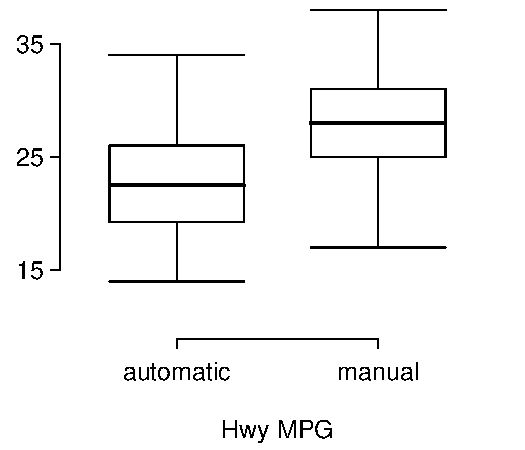
\includegraphics[width=0.7\textwidth]{ch_inference_for_means/figures/eoce/fuel_eff_hway/fuel_eff_hway_box.pdf}
\end{center}
\end{minipage}
}{}

% 29 - prison_isolation_T

\eoce{\qt{Prison isolation experiment, Part I\label{prison_isolation_T}}
Subjects from Central Prison in Raleigh, NC, volunteered
for an experiment involving an ``isolation'' experience.
The goal of the experiment was to find a treatment 
that reduces subjects' psychopathic deviant T scores.
This score measures a person's need for control or their rebellion against 
control, and it is part of a commonly used mental health test called the 
Minnesota Multiphasic Personality Inventory (MMPI) test. The experiment had 
three treatment groups: 
\begin{enumerate}[(1)]
\setlength{\itemsep}{0mm}
\item
    Four hours of sensory restriction plus a 15 minute
    ``therapeutic" tape advising that professional help
    is available.
\item
    Four hours of sensory restriction plus a 15 minute
    ``emotionally neutral'' tape on training hunting dogs.
\item
    Four hours of  sensory restriction but no taped message.
\end{enumerate}
Forty-two subjects were randomly assigned to these treatment groups, and an 
MMPI test was administered before and after the treatment. Distributions of the 
differences between pre and post treatment scores (pre - post) are shown below, 
along with some sample statistics. Use this information to independently test 
the effectiveness of each treatment. Make sure to clearly state your 
hypotheses, check conditions, and interpret results in the context of the data.\footfullcite{data:prison}

\begin{center}
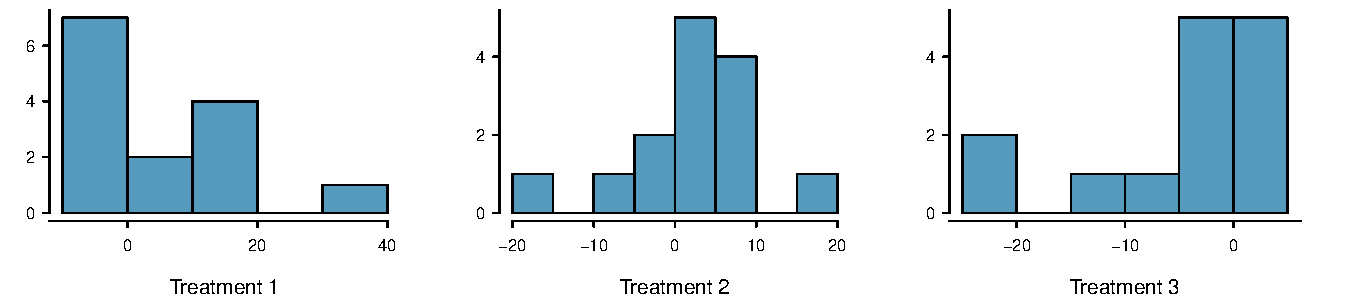
\includegraphics[width=\textwidth]{ch_inference_for_means/figures/eoce/prison_isolation_T/prison_isolation_hist} \\
$\:$ \\
\begin{tabular}{l  r  r  r  r  }
\hline
                & Tr 1  & Tr 2  & Tr 3      \\
\hline
Mean            & 6.21  & 2.86  & -3.21           \\
SD              & 12.3  & 7.94  & 8.57       \\
n               & 14        & 14        & 14     \\
\hline
\end{tabular}
\end{center}
}{}

% 30 - tf_compare_means

\eoce{\qt{True / False: comparing means\label{tf_compare_means}} Determine if the 
following statements are true or false, and explain your reasoning for 
statements you identify as false.
\begin{parts}
\item As the degrees of freedom increases, the $t$-distribution approaches 
normality.
\item We use a pooled standard error for calculating the standard error of the 
difference between means when sample sizes of groups are equal to each other.
\end{parts}
}{}
